\documentclass[aspectratio=169,11pt]{beamer}

\usepackage[utf8]{inputenc}
\usepackage[T1]{fontenc}
\usepackage{booktabs}
\usepackage{graphicx}

\usetheme{Madrid}

% --- TCS-inspired palette ---
\definecolor{nv}{RGB}{27,42,74}     % navy
\definecolor{bl}{RGB}{0,105,180}    % blue
\definecolor{mg}{RGB}{226,0,116}    % magenta
\definecolor{gr}{RGB}{138,148,166}  % gray

\setbeamercolor{structure}{fg=bl}
\setbeamercolor{frametitle}{bg=nv,fg=white}
\setbeamercolor{title}{fg=white}
\setbeamercolor{subtitle}{fg=white}
\setbeamercolor{author}{fg=white}
\setbeamercolor{date}{fg=white}
\setbeamercolor{title page header}{fg=white}
\setbeamercolor{block title}{bg=nv,fg=white}
\setbeamercolor{block body}{bg=white}
\setbeamercolor{block title example}{bg=bl,fg=white}
\setbeamercolor{block title alerted}{bg=mg,fg=white}
\setbeamercolor{alerted text}{fg=mg}
\setbeamercolor{itemize item}{fg=bl}
\setbeamercolor{itemize subitem}{fg=nv}
\setbeamercolor{enumerate item}{fg=bl}
\setbeamercolor{caption name}{fg=nv}
\setbeamercolor{footline}{fg=nv}

\setbeamertemplate{navigation symbols}{}
\setbeamertemplate{blocks}[rounded][shadow=false]
\setbeamerfont{title}{size=\Large,series=\bfseries}
\setbeamerfont{frametitle}{size=\large,series=\bfseries}

\title{\textbf{Generación autónoma de microservicios}}
\subtitle{Dónde está la industria · cómo funciona · qué cuesta · hacia dónde vamos}
\author{Ingeniería AgentIA}
\date{2026}

\begin{document}

{
\setbeamercolor{background canvas}{bg=nv}
\begin{frame}[plain]
  \titlepage
\end{frame}
}

\begin{frame}{Dónde está la industria: tres caminos}
  \begin{columns}[T]
    \begin{column}{0.33\textwidth}
      \begin{block}{1. Agentes generalistas de código}
        Arreglan o completan código \emph{ya existente}.
        \begin{itemize}
          \item Dominan los rankings.
          \item Saturados y \textbf{caros} (\$5--\$30 por tarea).
        \end{itemize}
      \end{block}
    \end{column}
    \begin{column}{0.33\textwidth}
      \begin{exampleblock}{2. Generadores guiados por especificación}
        Construyen la aplicación \emph{desde una especificación formal}.
        \begin{itemize}
          \item \textbf{Es nuestro camino.}
          \item Solo se resuelve \textbf{12--55\%}: mucho espacio.
        \end{itemize}
      \end{exampleblock}
    \end{column}
    \begin{column}{0.33\textwidth}
      \begin{block}{3. Agentes que se auto-mejoran}
        Escriben su propio ``manual'' de trabajo.
        \begin{itemize}
          \item Prometedor en laboratorio.
          \item En código real, mejora \textbf{casi nula}.
        \end{itemize}
      \end{block}
    \end{column}
  \end{columns}
  \vspace{1em}
  \centering
  \alert{\textbf{La lección de toda la investigación: el ingrediente que gana es una
  \emph{verificación} de fiar, no un modelo más listo.}}
\end{frame}

\begin{frame}{Cómo funciona la solución}
  \begin{center}
    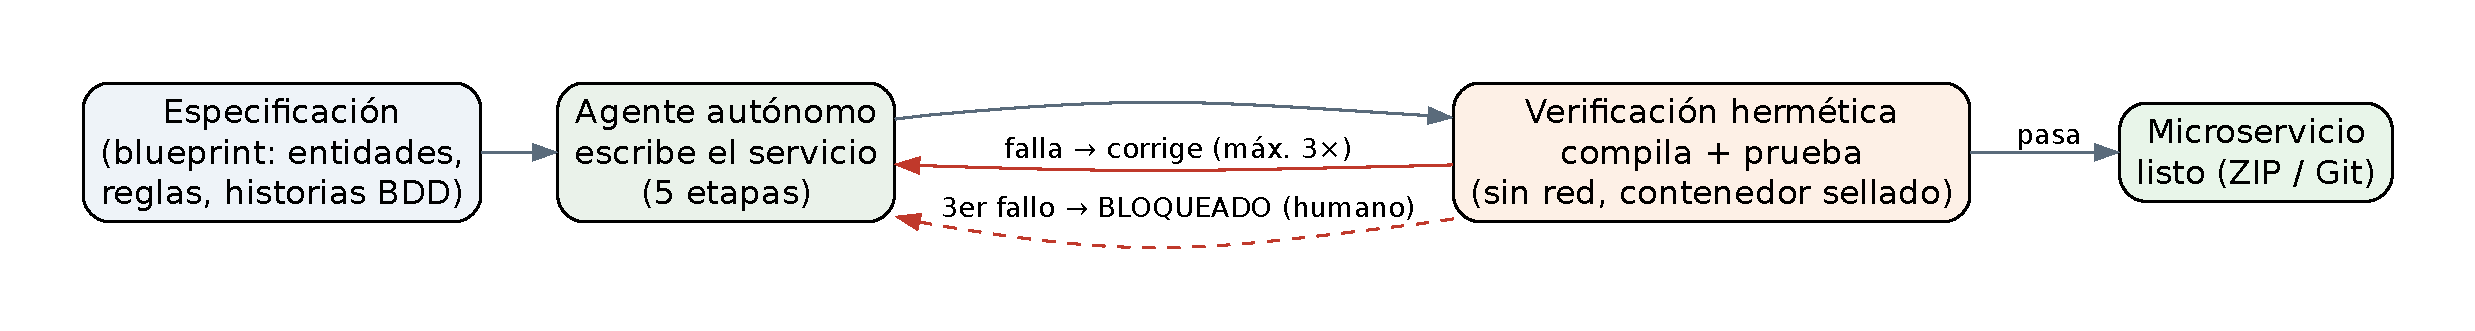
\includegraphics[width=0.96\textwidth]{fig/how_it_works.pdf}
  \end{center}
\end{frame}

\begin{frame}{El proceso, de punta a punta}
  \begin{center}
    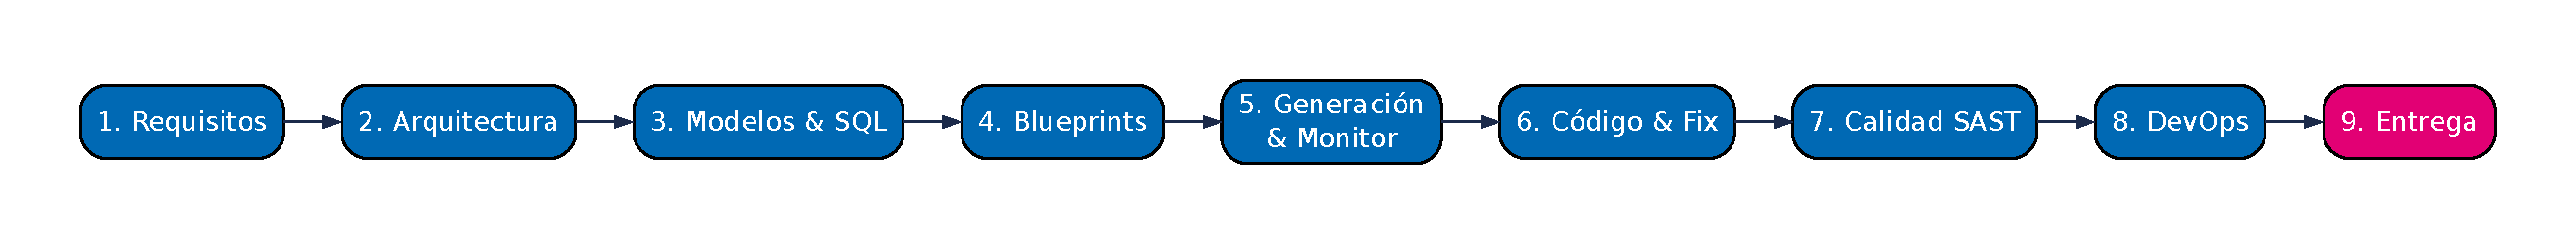
\includegraphics[width=\textwidth]{fig/lifecycle.pdf}
  \end{center}
  \vspace{0.4em}
  \centering Nueve etapas: de la especificación a la entrega (ZIP o Git), con
  generación y verificación en el centro.
\end{frame}

\begin{frame}{Lo que eso garantiza}
  \begin{itemize}
    \item \textbf{Se escribe} un servicio completo, no fragmentos: entidades, lógica,
    API, tests.
    \item \textbf{Se verifica} en un contenedor sellado, sin red: compila y pasa sus
    pruebas, o no se entrega.
    \item \textbf{Se autocorrige} hasta 3 veces; al tercer fallo se detiene y pide a
    un humano. Nunca un bucle infinito, nunca un ``éxito'' no comprobado.
    \item \textbf{Se audita} el cumplimiento de las reglas del proyecto, aplicadas por
    la plataforma, no por la opinión del modelo.
  \end{itemize}
\end{frame}

\begin{frame}{El coste (medido, sistema de registro + MLflow)}
  \begin{columns}
    \begin{column}{0.52\textwidth}
      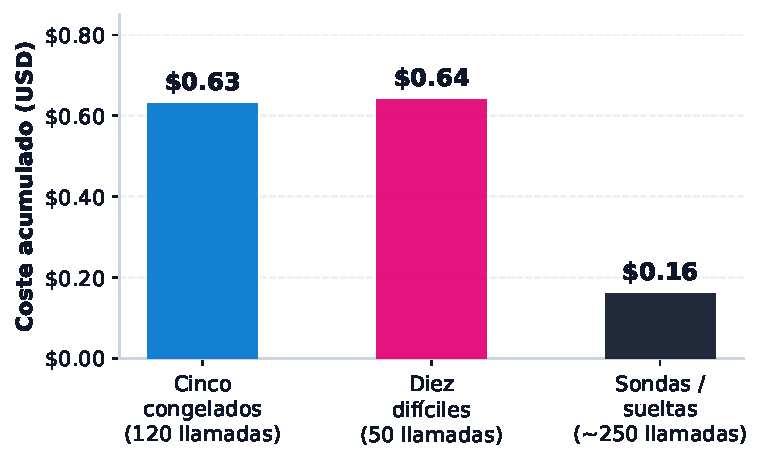
\includegraphics[width=\textwidth]{fig/cost_by_scope.pdf}
    \end{column}
    \begin{column}{0.44\textwidth}
      \begin{itemize}
        \item Un microservicio (dificultad media, recién ejecutado): \textbf{\$0.067}
        \item Rango por servicio: \$0.052 -- \$0.077
        \item Un servicio \textbf{garantizado} (se generan 3, se entrega el que
        compila): \textbf{\$0.20}
        \item \textbf{Total acumulado: \$8.15} en 1{,}219 llamadas
      \end{itemize}
    \end{column}
  \end{columns}
\end{frame}

\begin{frame}{Coste por etapa}
  \begin{center}
    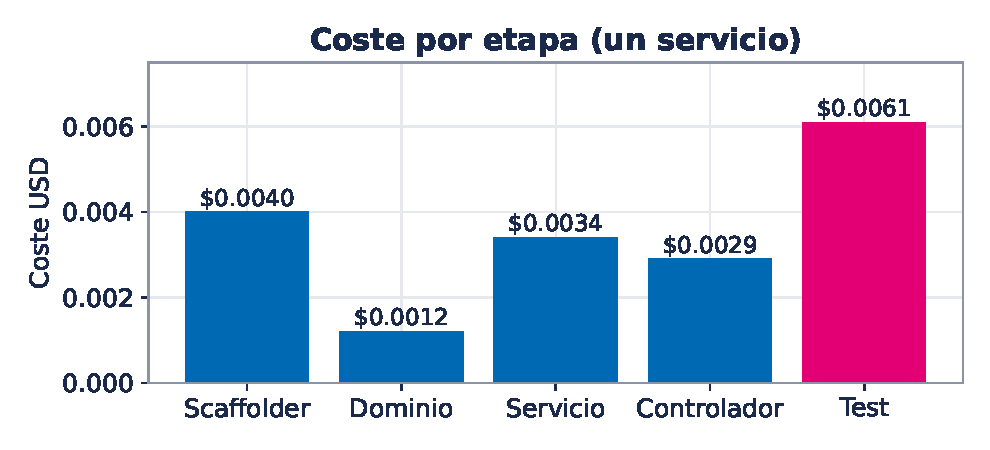
\includegraphics[width=0.62\textwidth]{fig/cost_by_stage.pdf}
  \end{center}
  \centering El test es la etapa más cara (\$0.0061); dominio la más barata (\$0.0012).
  El coste escala con el tamaño del servicio, de forma predecible.
\end{frame}

\begin{frame}{Tokens (último reporte de MLflow)}
  \begin{columns}
    \begin{column}{0.52\textwidth}
      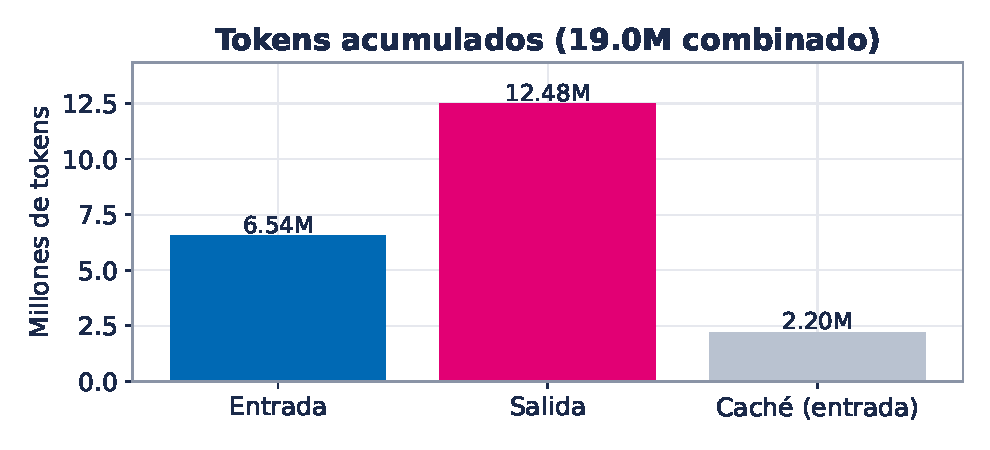
\includegraphics[width=\textwidth]{fig/tokens.pdf}
    \end{column}
    \begin{column}{0.44\textwidth}
      \begin{itemize}
        \item \textbf{19.0M tokens} combinados (registro)
        \item 6.5M entrada · 12.5M salida · 2.2M desde caché
        \item $\approx$\textbf{78K tokens por servicio}
        \item $\approx$15.6K por llamada; salida $\approx$1.9$\times$ la entrada
      \end{itemize}
    \end{column}
  \end{columns}
\end{frame}

\begin{frame}{El trabajo hecho hasta aquí}
  \begin{itemize}
    \item \textbf{La plataforma ya verifica su propia salida.} Antes reportaba ``0 de
    15 verificadas''; el bloqueo era un defecto de un carácter.
    \item \textbf{Ambas vías de producto compilan y prueban}, no solo una.
    \item \textbf{La métrica de calidad dejó de ser manipulable}.
    \item \textbf{El registro de coste es honesto} y visible en MLflow.
    \item Queda \textbf{un punto abierto}: el verificador a veces cambia su veredicto
    (se corrige en la siguiente iteración).
  \end{itemize}
\end{frame}

\begin{frame}{El futuro: auto-mejora}
  \begin{block}{La idea}
    Que el sistema aprenda de sus propios errores y mejore su ``manual'' de
    generación automáticamente.
  \end{block}
  \begin{alertblock}{Lo que la evidencia exige}
    \emph{Un sistema que aprende de un juez ruidoso aprende ruido.} Por eso el orden
    correcto es:
  \end{alertblock}
  \begin{enumerate}
    \item Hacer \textbf{sólido el verificador}.
    \item Hacer que la \textbf{medida detecte} los fallos reales.
    \item \emph{Solo entonces}, encender el bucle de auto-mejora.
  \end{enumerate}
  El mecanismo de auto-mejora \textbf{ya está construido}; se enciende cuando la base
  sea fiable.
\end{frame}

\begin{frame}{El camino}
  \begin{center}
    \begin{tabular}{lll}
      \toprule
      \textbf{Paso} & \textbf{Qué} & \textbf{Esfuerzo} \\
      \midrule
      1 & Sólido el verificador (una configuración) & corto \\
      2 & Detectar fallos reales en la medida & corto \\
      3 & Medir si un ``manual'' aporta & \$3--\$5 \\
      4 & Encender la auto-mejora (ya construida) & condicionado \\
      \bottomrule
    \end{tabular}
  \end{center}
  \begin{block}{El mensaje}
    De ``no podía verificar su propia salida'' a ``genera, compila y verifica por
    \$0.07, y se auto-mejorará cuando la base sea fiable''.
  \end{block}
\end{frame}

\end{document}
